\documentclass[11pt,a4paper]{jsarticle}

\usepackage{amsmath,amssymb}
\usepackage{bm}
\usepackage{graphicx}
\usepackage{ascmac}
\usepackage{subfigure}
\newlength{\subfigwidth}
\newlength{\subfigcolsep}

\graphicspath{{./img/}}

\title{TPC-H performance measure}
\author{Keisuke Suzuki}

\begin{document}
\maketitle
\section{実験環境}
\begin{itemize}
 \item CPU : Xeon X7560 @ 2.27GHz x4
 \item Memory : 64GB
 \item DBMS : PostgreSQL 9.2
 \item RAID0 : iodrive x8 (chunk size = 64KB)
 \item 各テーブルのprimary key上にB-tree indexを構築
 \item Scale Factor = 100
 \item shared buffer = 8GB
\end{itemize}

\clearpage
\section{Query 8}
簡単の為、Query8のうちのI/Oがメインとなる部分のみを実行する。
work\_memの値(ひとつのsortやhash tableに使用されるメモリサイズ)を変化させて、実行時間を計測する。

\subsection{Query and Execution Plan}
\begin{verbatim}
 select
	extract(year from o_orderdate) as o_year,
	l_extendedprice * (1 - l_discount) as volume,
	n2.n_name as nation
from
	part, supplier, lineitem, orders,
	customer, nation n1, nation n2,	region
where
	p_partkey = l_partkey
	and s_suppkey = l_suppkey
	and l_orderkey = o_orderkey
	and o_custkey = c_custkey
	and c_nationkey = n1.n_nationkey
	and n1.n_regionkey = r_regionkey
	and r_name = 'AMERICA'
	and s_nationkey = n2.n_nationkey
	and o_orderdate between date '1995-01-01' and date '1996-12-31'
	and p_type = 'ECONOMY ANODIZED STEEL'
\end{verbatim}

\begin{figure}[thbp]
 \begin{center}
  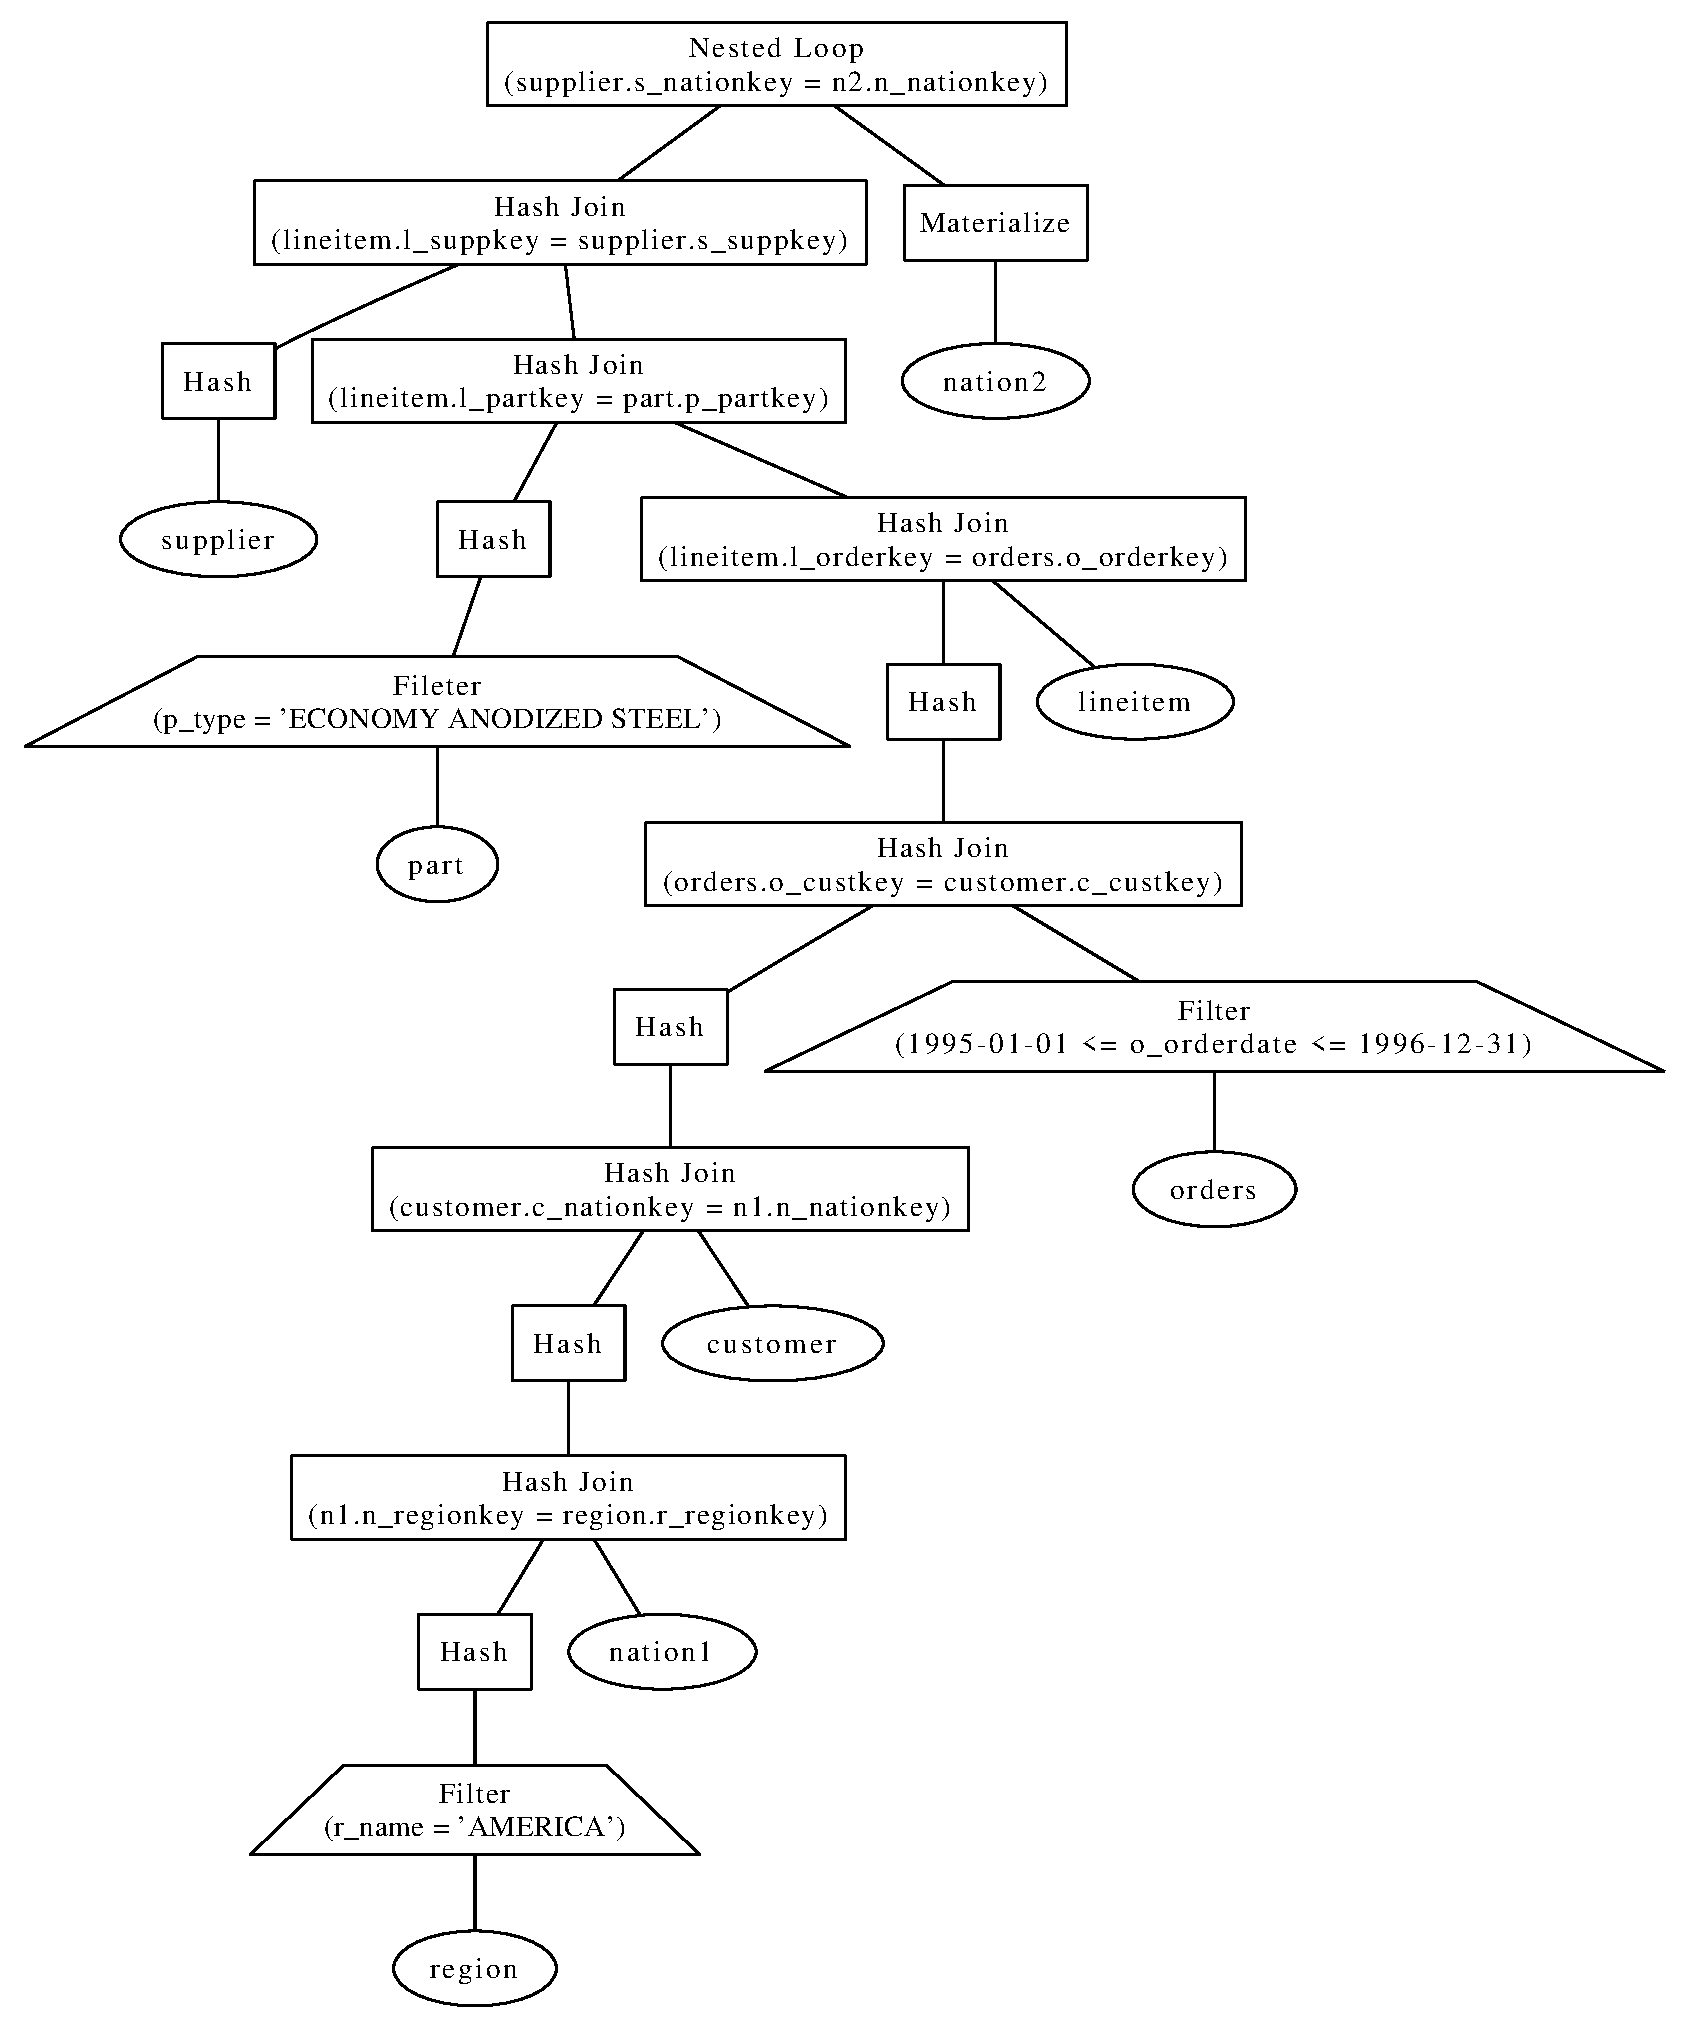
\includegraphics[width=150mm]{query8.eps}
 \end{center}
 \caption{Query 8 execution plan}
 \label{fig:query8}
\end{figure}

\clearpage
\subsection{work\_mem = 64kB - 2GB}
\begin{figure}[thbp]
 \begin{center}
  \includegraphics[width=95mm]{q8cputime.eps}
 \end{center}
 \caption{Executinon time and breakdown by mpstat}
 \label{fig:q8cputime}
\end{figure}

\begin{figure}[thbp]
 \begin{center}
  \includegraphics[width=95mm]{q8exectime.eps}
 \end{center}
 \caption{Executinon time and I/O cost and CPU cost}
 \label{fig:q8exectime}
\end{figure}

\begin{verbatim}
+   2.81%         postgres  postgres                 [.] heap_fill_tuple
+   1.43%         postgres  postgres                 [.] heap_form_minimal_tuple
+   1.05%         postgres  postgres                 [.] BufFileWrite
+   0.50%         postgres  postgres                 [.] ExecStoreMinimalTuple
...
\end{verbatim}

\subsection{work\_mem = 16MB - 32MB}
\begin{figure}[thbp]
 \begin{center}
  \includegraphics[width=95mm]{q8_16_32_cputime.eps}
 \end{center}
 \caption{Executinon time and breakdown by mpstat}
 \label{fig:q8cputime1632}
\end{figure}

\begin{figure}[thbp]
 \begin{center}
  \includegraphics[width=95mm]{q8_16_32_exectime.eps}
 \end{center}
 \caption{Executinon time and I/O cost and CPU cost}
 \label{fig:q8exectime1632}
\end{figure}

\clearpage
\section{join between orders and lineitem}
\subsection{work\_mem = 64kB - 8GB}
\begin{figure}[thbp]
 \begin{center}
  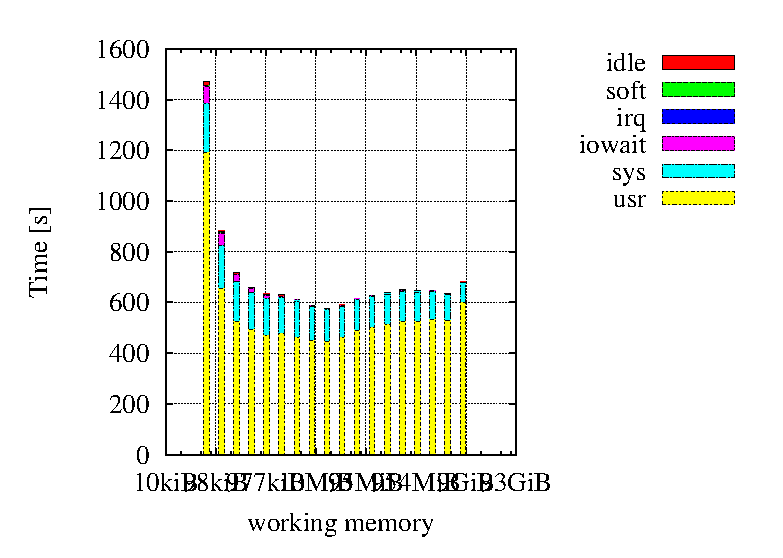
\includegraphics[width=95mm]{oljoincputime.eps}
 \end{center}
 \caption{Executinon time and breakdown by mpstat}
 \label{fig:q8cputime}
\end{figure}

\begin{figure}[thbp]
 \begin{center}
  \includegraphics[width=95mm]{oljoinexectime.eps}
 \end{center}
 \caption{Executinon time and I/O cost and CPU cost}
 \label{fig:q8exectime}
\end{figure}

\end{document}
